\documentclass[11pt,a4paper]{article}
\usepackage[margin=1in]{geometry}
\usepackage{graphicx}
\title{Network Structure of ERC8004 Reputation Flows on Ethereum:\\A Science-Chief Review of Q3\_v2}
\author{Science-Chief}
\date{2026-03-08}
\begin{document}
\maketitle

\begin{abstract}
This report presents a full scientific interpretation of the Q3\_v2 network milestone for ERC8004 feedback dynamics on Ethereum. Starting from on-chain feedback events, we model the system as a bipartite client-to-agent graph, derive an agent projection, estimate centrality profiles, detect communities, evaluate temporal stability, and test structural signals against null-model baselines. The core objective is to determine whether reputation production is broadly distributed or structurally concentrated. The evidence indicates a non-trivial network organization with visible concentration and mesoscale structure; however, inferential strength is not yet uniformly strong across all significance checks. Therefore, the current state supports internal scientific progression while recommending caution for strong external claims.
\end{abstract}

\section{Introduction}
The central question in this study is not merely how many feedback events exist in the ERC8004 ecosystem, but whether those events generate a robust reputation fabric. A system can accumulate many interactions while still remaining structurally fragile if those interactions are concentrated in a small subset of actors. In reputation systems, this distinction is fundamental: volume alone is insufficient, while topology reveals resilience, diversity, and potential bias channels.

In the ERC8004 setting, identity and reputation are represented through distinct on-chain registries. This architecture is ideal for a network-science analysis because each feedback event is an explicit relational edge between an evaluator and an evaluated entity. The purpose of Q3\_v2 is therefore to move beyond descriptive counts and establish a structured inferential layer: centrality, community organization, persistence over time, and contrast against randomized baselines.

\section{Data Provenance and Extraction Context}
The analyzed events come from ERC8004 Ethereum registries. Identity-side references are anchored at \texttt{0x8004A169FB4a3325136EB29fA0ceB6D2e539a432}, while reputation flows are sourced from \texttt{0x8004BAa17C55a88189AE136b182e5fdA19dE9b63}. The primary input for Q3\_v2 is the event table \texttt{reputation\_newfeedback.csv}, where each row records a feedback interaction and includes block index, agent identifier, client address, and payload fields.

The extraction strategy preserves event-level fidelity. Rather than collapsing observations prematurely, the pipeline first reconstructs a weighted interaction graph and only then derives aggregate network descriptors. This order is important: it prevents loss of topological information and keeps interpretability tied to the original on-chain event structure.

\section{Methods}
We begin with a bipartite graph whose left partition is composed of client addresses and whose right partition is composed of agent identifiers. A weighted edge is assigned whenever a client submits one or more feedback events to an agent; edge weight equals interaction multiplicity.

From this bipartite representation, we construct an agent-projection graph based on shared evaluators. Intuitively, two agents are close when they are evaluated by overlapping client sets. We retain both raw overlap and normalized similarity signals in the projection output.

We then compute multi-metric centrality: weighted degree (interaction mass), betweenness (brokerage role), and PageRank (global structural relevance). Community detection is applied to identify mesoscale organization. Temporal stability is assessed using block-window slices and overlap@20 of top-central nodes between adjacent windows. Finally, null-model Monte Carlo runs (100 simulations) are used to estimate whether selected structural statistics exceed random expectations under constrained rewiring.

\section{Results}
Technical integrity checks pass. The bipartite edge table contains 2,251 weighted pairs, and the sum of edge weights equals 2,776, matching the event count target for consistency. The centrality table contains 1,461 agents with no duplicate identifiers, supporting deterministic downstream ranking.

Figure~\ref{fig:deg} shows the degree-distribution profile. The shape is right-skewed and consistent with concentration, meaning that participation intensity is unevenly distributed. Figure~\ref{fig:cent} confirms this from a ranking perspective: top-central entities accumulate disproportionate structural relevance.

Figure~\ref{fig:comm} displays community-size distribution and provides first evidence of mesoscale segmentation. The presence of multiple communities suggests that the feedback ecosystem is not a uniform random cloud but exhibits organized substructure.

Temporal persistence is summarized in Figure~\ref{fig:temp}. Overlap signals indicate that a subset of structurally relevant agents remains recurrent across slices, although persistence is not perfectly rigid. This is compatible with a mixed regime where a stable core coexists with a variable periphery.

Finally, Figure~\ref{fig:null} reports null-model comparison. The key conclusion is nuanced: structural signals are visible, but significance is not uniformly strong across all tested statistics in this baseline run. This is sufficient for internal advancement but not yet for aggressive external inference.

\begin{figure}[htbp]
\centering
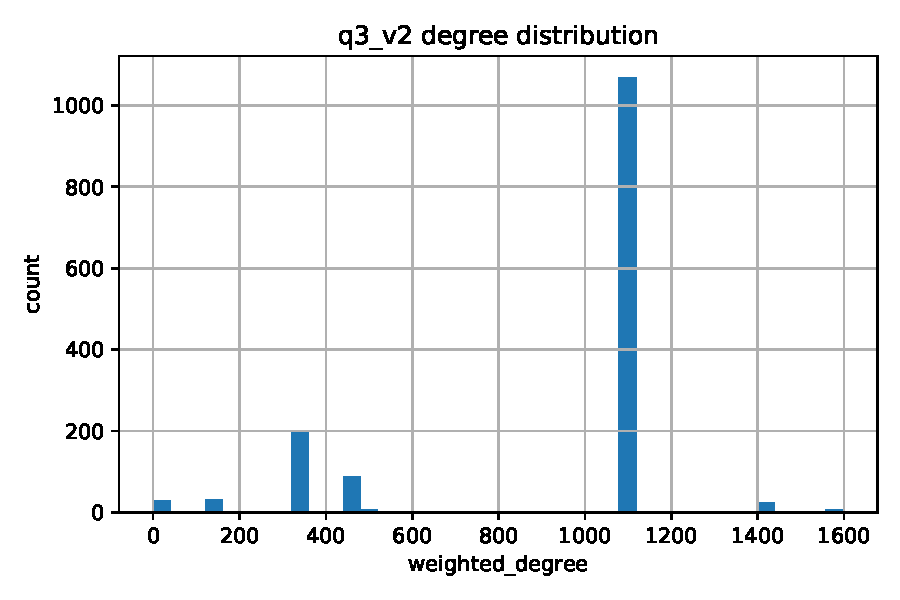
\includegraphics[width=0.86\textwidth]{figures/q3_v2_degree_distribution.pdf}
\caption{Degree distribution in the Q3\_v2 network representation.}
\label{fig:deg}
\end{figure}

\begin{figure}[htbp]
\centering
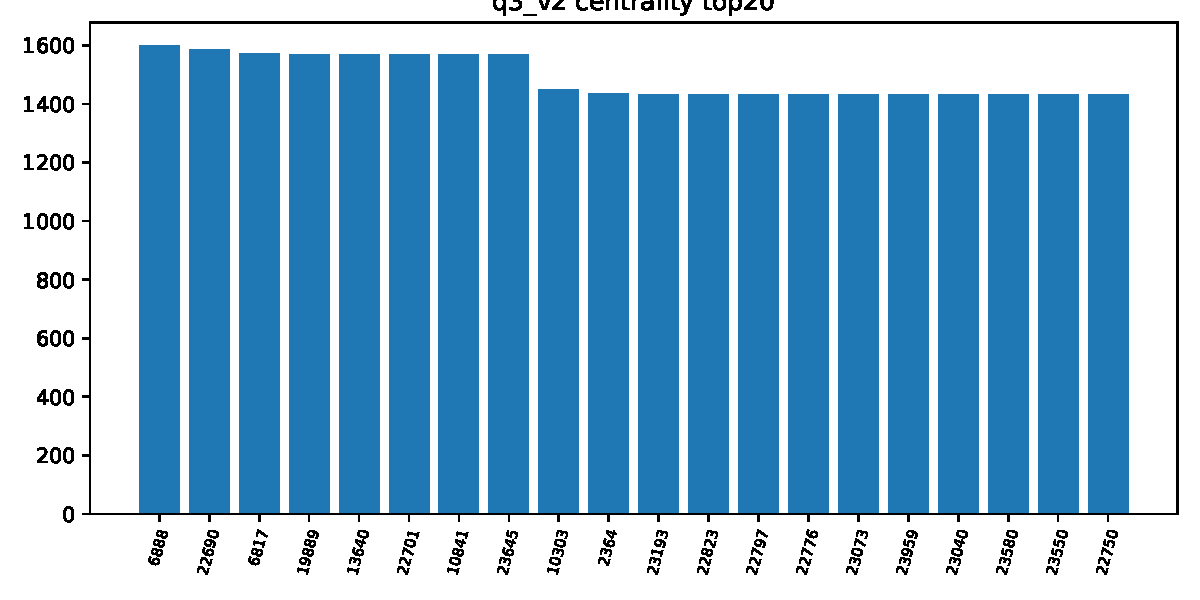
\includegraphics[width=0.86\textwidth]{figures/q3_v2_centrality_top20.pdf}
\caption{Top-20 agents by centrality profile.}
\label{fig:cent}
\end{figure}

\begin{figure}[htbp]
\centering
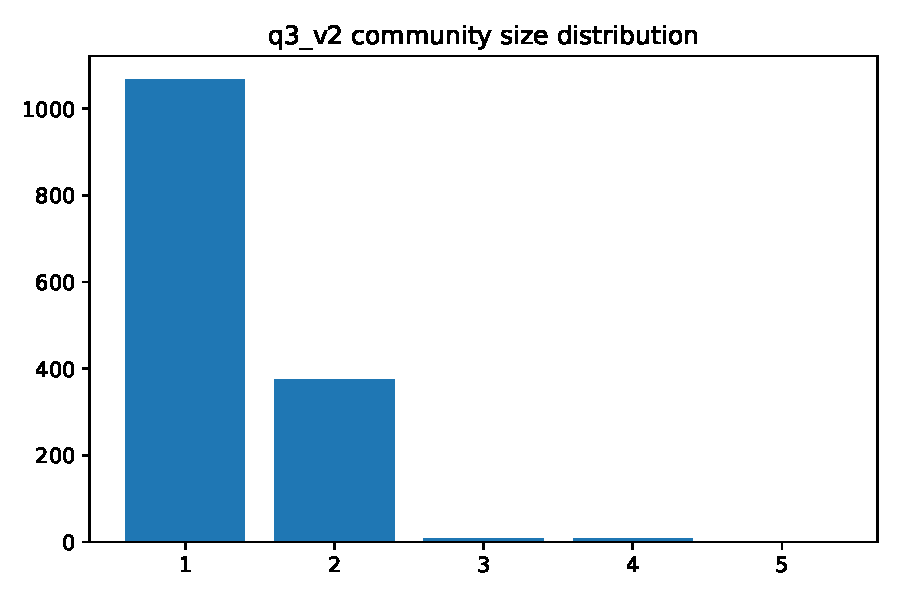
\includegraphics[width=0.86\textwidth]{figures/q3_v2_community_size_distribution.pdf}
\caption{Community-size distribution in the projected agent graph.}
\label{fig:comm}
\end{figure}

\begin{figure}[htbp]
\centering
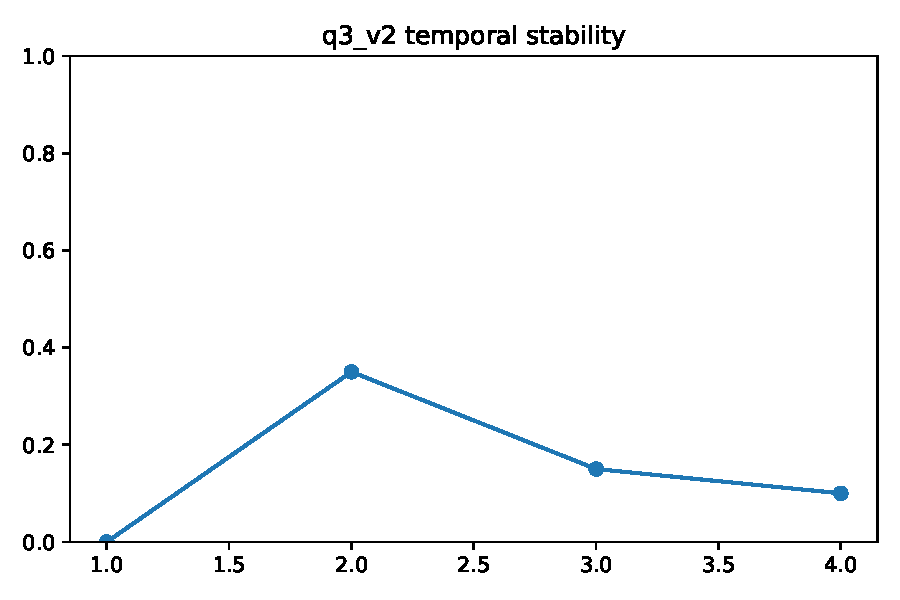
\includegraphics[width=0.86\textwidth]{figures/q3_v2_temporal_stability.pdf}
\caption{Temporal stability across block-window slices (overlap-based).}
\label{fig:temp}
\end{figure}

\begin{figure}[htbp]
\centering
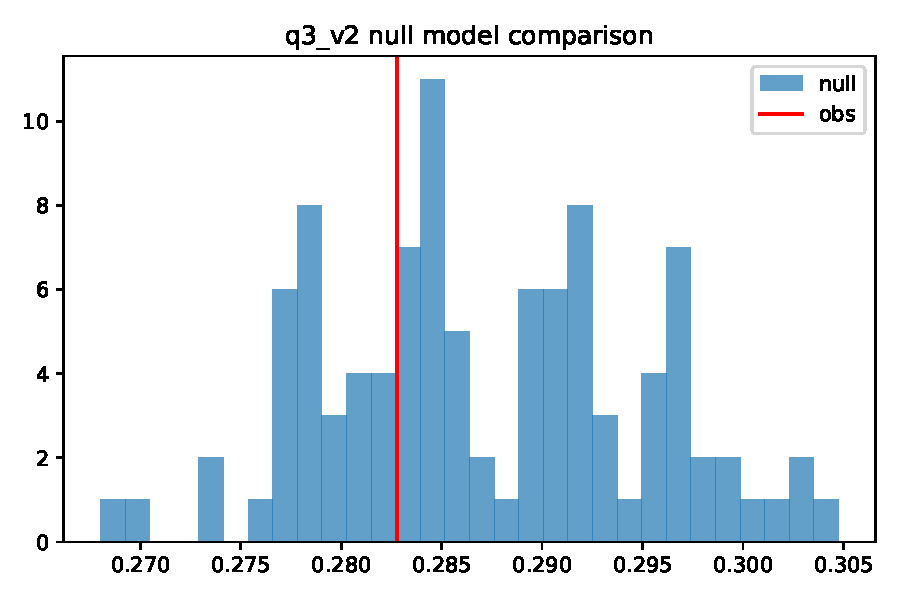
\includegraphics[width=0.86\textwidth]{figures/q3_v2_null_model_comparison.pdf}
\caption{Observed structure compared with null-model baselines.}
\label{fig:null}
\end{figure}

\section{Discussion}
The Q3\_v2 milestone substantially improves inferential quality relative to the previous micro cut. The analysis now captures not only who receives feedback, but also how relational structure is organized, how stable that structure is, and how far it departs from random baselines.

Scientifically, the current picture is coherent with a concentrated-yet-structured reputation layer. This is an important distinction: concentration alone could be interpreted as fragility, but concentration accompanied by persistent mesoscale organization may indicate emerging specialization or role differentiation. Determining which interpretation dominates requires deeper robustness.

The practical implication is that policy or product interventions should not rely only on event totals. They should target structural objectives such as evaluator diversity, reduction of centrality over-dependence, and healthier cross-community connectivity.

\section{Limitations}
The present milestone remains Ethereum-only, which limits ecosystem-level generalization. Projection results are sensitive to weighting definitions, and null-model depth (100 runs) is a baseline rather than publication-grade strength for all inferential dimensions. Temporal slicing is also coarse, so fine-grained regime transitions may be under-resolved.

\section{Conclusion}
Q3\_v2 delivers a valid and reproducible network-inference foundation for ERC8004 analysis. The evidence supports progression to advanced internal research and integration with activation-lag and semantic modules. At the same time, external claims should remain calibrated until robustness is strengthened through richer null-model testing, weighting sensitivity analysis, and finer temporal diagnostics.

\section*{Appendix: Source Paths}
\textbf{Figures}\\
\begin{itemize}
\item \texttt{workspaces/science-chief/outbox/Reports/Q3\_V2\_NETWORK\_INFERENCE\_PACK\_2026-03-08/figures/q3\_v2\_degree\_distribution.pdf}
\item \texttt{workspaces/science-chief/outbox/Reports/Q3\_V2\_NETWORK\_INFERENCE\_PACK\_2026-03-08/figures/q3\_v2\_centrality\_top20.pdf}
\item \texttt{workspaces/science-chief/outbox/Reports/Q3\_V2\_NETWORK\_INFERENCE\_PACK\_2026-03-08/figures/q3\_v2\_community\_size\_distribution.pdf}
\item \texttt{workspaces/science-chief/outbox/Reports/Q3\_V2\_NETWORK\_INFERENCE\_PACK\_2026-03-08/figures/q3\_v2\_temporal\_stability.pdf}
\item \texttt{workspaces/science-chief/outbox/Reports/Q3\_V2\_NETWORK\_INFERENCE\_PACK\_2026-03-08/figures/q3\_v2\_null\_model\_comparison.pdf}
\end{itemize}

\textbf{Tables}\\
\begin{itemize}
\item \texttt{workspaces/science-chief/outbox/Reports/Q3\_V2\_NETWORK\_INFERENCE\_PACK\_2026-03-08/tables/q3\_v2\_bipartite\_edges\_weighted.csv}
\item \texttt{workspaces/science-chief/outbox/Reports/Q3\_V2\_NETWORK\_INFERENCE\_PACK\_2026-03-08/tables/q3\_v2\_agent\_projection\_weighted.csv}
\item \texttt{workspaces/science-chief/outbox/Reports/Q3\_V2\_NETWORK\_INFERENCE\_PACK\_2026-03-08/tables/q3\_v2\_agent\_centrality.csv}
\item \texttt{workspaces/science-chief/outbox/Reports/Q3\_V2\_NETWORK\_INFERENCE\_PACK\_2026-03-08/tables/q3\_v2\_community\_membership.csv}
\item \texttt{workspaces/science-chief/outbox/Reports/Q3\_V2\_NETWORK\_INFERENCE\_PACK\_2026-03-08/tables/q3\_v2\_temporal\_stability.csv}
\item \texttt{workspaces/science-chief/outbox/Reports/Q3\_V2\_NETWORK\_INFERENCE\_PACK\_2026-03-08/tables/q3\_v2\_null\_model\_test.csv}
\item \texttt{workspaces/science-chief/outbox/Reports/Q3\_V2\_NETWORK\_INFERENCE\_PACK\_2026-03-08/tables/q3\_v2\_top20\_multi\_metric.csv}
\end{itemize}

\end{document}
